\documentclass[12pt,a4paper]{article}
\usepackage[a4paper, margin=2cm]{geometry}
\usepackage{amsmath}
\usepackage{fancyhdr}
\usepackage{graphicx}
\usepackage{pdflscape}
\usepackage{svg}
\usepackage{hyperref}
\usepackage{enumitem}
\usepackage[absolute,overlay]{textpos}
\usepackage{lipsum}
\usepackage{amssymb}

\usepackage[portuguese]{babel}
\usepackage{lmodern}
\renewcommand*{\familydefault}{\sfdefault}
\usepackage{geometry}
\usepackage{setspace}
\usepackage{xcolor}
\usepackage{tikz}
\definecolor{col1}{RGB}{0,160,255}
\definecolor{col2}{RGB}{7,74,163}
\usepackage{setspace}
\usepackage{listings}
\usepackage{titlesec}
\usepackage{color}
\usepackage{textgreek}

\newcommand{\reporttitle}{Projeto Computacional - 1.ª Parte}
\newcommand{\authorgroup}{Grupo 16 - Afonso Ribeiro, Diogo Rodrigues, Pedro Mendes}
\newcommand{\istul}{Instituto Superior Técnico -- Universidade de Lisboa}
\newcommand{\reportcourse}{Matemática Experimental}
\newcommand{\reportyear}{2024/2025}

\newcommand{\m}[1]{\mathbf{#1}}

\hypersetup{
    colorlinks=true,
    linkcolor=blue,
    filecolor=magenta,
    urlcolor=blue,
    citecolor=blue,
    pdftitle={\reporttitle},
    pdfpagemode=FullScreen,
}

\pagestyle{fancy}
\fancyhf{}
\lhead{\reporttitle}
\rhead{\reportcourse}
\lfoot{\authorgroup}
\rfoot{\thepage}


\renewcommand{\footrulewidth}{0.2pt}

\renewcommand\thesection{\arabic{section}.}
\renewcommand\thesubsection{\thesection\arabic{subsection}.}
\renewcommand\thesubsubsection{\thesubsection\arabic{subsubsection}.}

\usepackage{etoolbox} % Necessário para modificar comandos
\makeatletter % Indentar parágrafos dentro de subseções
\preto\subsection{\setlength{\parindent}{2em}} % Ajusta o tamanho do recuo
\makeatother

\begin{document}
    \begin{titlepage}
        \thispagestyle{empty}
        \newgeometry{left=2cm, right=1.5cm, top = 2cm, bottom=2cm}
        \begin{tikzpicture}[overlay, fill opacity=0.7]
        \fill[col1] (12,-27) rectangle (15,4);
        \rotatebox{-45}{\fill[col2] (12, -23) rectangle (21,20);}
        \node[anchor=base, color=white] at (13.50, 0) {\Huge \textbf{M}};
        \node[anchor=base, color=white] at (13.50, -1) {\Huge \textbf{A}};
        \node[anchor=base, color=white] at (13.50, -2) {\Huge \textbf{T}};
        \node[anchor=base, color=white] at (13.50, -3) {\Huge \textbf{E}};
        \node[anchor=base, color=white] at (13.50, -4) {\huge \textbf{M}};
        \node[anchor=base, color=white] at (13.50, -5) {\huge \textbf{Á}};
        \node[anchor=base, color=white] at (13.50, -6) {\Huge \textbf{T}};
        \node[anchor=base, color=white] at (13.50, -7) {\Huge \textbf{I}};
        \node[anchor=base, color=white] at (13.50, -8) {\Huge \textbf{C}};
        \node[anchor=base, color=white] at (13.50, -9) {\Huge \textbf{A}};
        \node[anchor=base] at (13.50, -11.7) {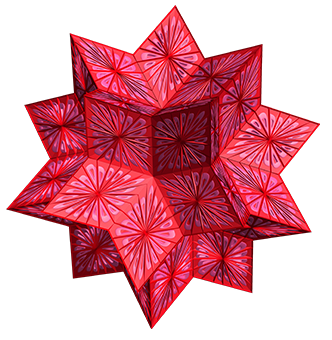
\includegraphics[width=2cm]{Mathematica.png}};
        \node[anchor=base, color=white] at (13.50, -13) {\Huge \textbf{E}};
        \node[anchor=base, color=white] at (13.50, -14) {\Huge \textbf{X}};
        \node[anchor=base, color=white] at (13.50, -15) {\Huge \textbf{P}};
        \node[anchor=base, color=white] at (13.50, -16) {\Huge \textbf{E}};
        \node[anchor=base, color=white] at (13.50, -17) {\Huge \textbf{R}};
        \node[anchor=base, color=white] at (13.50, -18) {\Huge \textbf{I}};
        \node[anchor=base, color=white] at (13.50, -19) {\huge \textbf{M}};
        \node[anchor=base, color=white] at (13.50, -20) {\Huge \textbf{E}};
        \node[anchor=base, color=white] at (13.50, -21) {\Huge \textbf{N}};
        \node[anchor=base, color=white] at (13.50, -22) {\Huge \textbf{T}};
        \node[anchor=base, color=white] at (13.50, -23) {\Huge \textbf{A}};
        \node[anchor=base, color=white] at (13.50, -24) {\Huge \textbf{L}};
        
        \node[anchor=center, color=black, rotate=45] at (5, -10.9) {\Huge \textbf{RELATÓRIO}};
        \end{tikzpicture}
        \begin{spacing}{1.5}
        \begin{flushleft}
        {\Huge \textbf{Projeto Computacional}}\\ [10pt]
        {\huge  \textbf{1.ª Parte}}\\ [48pt]
        {
\includegraphics[scale=0.40]{IST_Logo.png}} \\ [1.5cm]
        \end{flushleft}
        \end{spacing}
        \begin{minipage}{2cm}
        \end{minipage} 
        \vspace{6.4 cm}
        \begin{flushleft}
        
        \Large \textcolor{white}{
            Trabalho realizado por: \\
            Afonso Ribeiro, ist1102763 \\
            Diogo Rodrigues, ist1113787 \\
            Pedro Mendes, ist1109994 \\
            \vspace{0.5cm} \\
            Com o apoio dos professores: \\
            Pedro Lima \\
            André Crispim
        }
        \end{flushleft}
        \vspace{1cm}
     \end{titlepage}

    \setcounter{page}{2}
    \setcounter{secnumdepth}{0} % Disable numbering for sections and below
    \setlength{\parskip}{0em}

    \newlength{\imagewidth} % Declare a new length
    \setlength{\imagewidth}{8cm} % Set its value


    \section{1. Número de Trigg}
    \subsection{a)}
        \begin{itemize}
            \item \texttt{HasDistinctDig[n\_Integer] /; IntegerLength[n] <= 4 := \\ If[IntegerLength[n] == 4, \\ Length[Union[IntegerDigits[n]]] > 1, \\ True]}
        \end{itemize}
        
        A função \textbf{FourDifDig} recebe como argumento um número inteiro constituído por quatro algarismos, no máximo. Se o operador atribuir à função um número inteiro constituído exatamente por quatro dígitos, com primeiro dígito não nulo (IntegerLength[n]==4), a função converte o número fornecido para uma lista dos seus dígitos decimais (IntegerDigits[n]), na qual foram eliminados todos os algarismos duplicados utilizando o comando Union. A função avalia se o número dado é constituído por algarismos todos iguais, vendo se o comprimento (Length) da lista criada é maior do que 1. Se este for maior que 1, o número não é formado por quatro dígitos iguais. Se o número introduzido for constituído por menos de quatro dígitos com primeiro dígito não nulo, a função avalia esse número com True (de seguida vamos querer adicionar zeros à esquerda até o número ter 4 dígitos. Assim, esse número nunca terá 4 dígitos iguais.

        \begin{itemize}
            \item \texttt{FilteredList = Select[Range[9999], HasDistinctDig];}
        \end{itemize}
        
        A função \texttt{FilteredList} seleciona da lista de todos os números inteiros de 1 a 9999 aqueles que não têm dígitos todos iguais.

        \begin{itemize}
            \item \texttt{DigList[n\_Integer]:= IntegerDigits[n,10,4]}
        \end{itemize}
        
        A função \texttt{DigList} recebe como argumento um número inteiro. Ela converte o número dado pelo operador para uma lista dos seus dígitos na base decimal, garantindo que o número tem um comprimento fixo. Ou seja, se a representação do número introduzido tiver menos de quatro dígitos, o mesmo é preenchido com zeros à esquerda até ser constituído por quatro dígitos.

        \begin{itemize}
            \item \texttt{N4 = Map[DigList, FilteredList];}
        \end{itemize}
        
        A função \texttt{N4} aplica a função \texttt{DigList} a todos os elementos de \texttt{FilteredList}, devolvendo uma lista de sublistas, cada uma constituída pelos dígitos dos números pertencentes a \texttt{N4}.

        \begin{itemize}
            \item \texttt{Length[N4]}
        \end{itemize}
        
        O comando \texttt{Length[N4]} devolve o comprimento da lista \texttt{N4}, ou seja, indica quantos números constituem o conjunto \texttt{N4}.

    \subsection{b)}
        \begin{itemize}
            \item \texttt{alfa[n\_Integer]:= Sort[IntegerDigits[n,10,4]][[4]]}
            \item \texttt{beta[n\_Integer]:= Sort[IntegerDigits[n,10,4]][[3]]}
            \item \texttt{gamma[n\_Integer]:= Sort[IntegerDigits[n,10,4]][[2]]}
            \item \texttt{delta[n\_Integer]:= Sort[IntegerDigits[n,10,4]][[1]]}
        \end{itemize}
        
        Cada uma destas funções recebe como argumento um número inteiro. Cada uma delas devolve o i-ésimo algarismo da lista dos dígitos do número introduzido organizada por ordem crescente.

        \begin{itemize}
            \item \texttt{T[n\_Integer]:= FromDigits[{beta[n], alfa[n], delta[n], gamma[n]}] \\ - FromDigits[Reverse[{beta[n], alfa[n], delta[n], gamma[n]}]]}
        \end{itemize}
        
        A função \texttt{T} recebe como argumento um número inteiro. Ela efetua a diferença entre dois números inteiros construídos a partir de uma lista ordenada de forma diferente. No primeiro número, os algarismos que ocupam as posições 1 e 3 trocam, entre si, de posição, e o mesmo acontece com os algarismos que ocupam as posições 2 e 4. No segundo número, a ordem dos algarismos é invertida em relação ao primeiro.
        
        \begin{itemize}
            \item \texttt{T[1023]}
            \item \texttt{T[1234]}
            \item \texttt{T[5626]}
        \end{itemize}
        
        Os comandos \texttt{T[1023]}, \texttt{T[1234]} e \texttt{T[5626]} calculam a imagem dos números 1023, 1234 e 5626, respetivamente, pela função \texttt{T}.

    \subsection{c)}
        \begin{itemize}
            \item \texttt{FindFixedPoint[n\_Integer]:= NestWhile[T, n, Function[x, T[x]!=x]]}
        \end{itemize}
        
        A função \texttt{FindFixedPoint} recebe como argumento um número inteiro. Partindo do número introduzido, a função \texttt{T} é iterada sucessivas vezes até que a condição \texttt{T[x]!=x} seja falsa, ou seja, até encontrar o seu ponto fixo. A função \texttt{FindFixedPoint} devolve o ponto fixo do número introduzido.

        \textbf{Nota}: A função FindFixedPoint está bem definida para qualquer número pertencente a N4 (todos os números pertencentes a N4 têm ponto fixo).
        
        \begin{itemize}
            \item \texttt{IterList[n\_Integer]:= NestWhileList[T, n, Function[x, T[x]!=x]]}
        \end{itemize}
        
        A função \texttt{IterList} recebe como argumento um número inteiro. Partindo do número introduzido, a função \texttt{T} é iterada sucessivas vezes até que a condição \texttt{T[x]!=x} seja falsa. A função \texttt{IterList} devolve uma lista que contém os números obtidos em cada iteração.

        \begin{itemize}
            \item \texttt{FindFixedPoint[1023]}
            \item \texttt{IterList[1023]}
            \item \texttt{FindFixedPoint[1234]}
            \item \texttt{IterList[1234]}
            \item \texttt{FindFixedPoint[5626]}
            \item \texttt{IterList[5626]}
        \end{itemize}
        
        Os comandos \texttt{FindFixedPoint[1023]}, \texttt{FindFixedPoint[1234]} e \texttt{FindFixedPoint[5626]} devolvem todos o número 2538, ou seja, o ponto fixo de 1023, 1234 e 5626 é 2538. Os comandos \texttt{IterList[1023]} e \texttt{IterList[1234]} devolvem, respetivamente, as listas \{1023, 1269, 4716, 2538\} e \{1234, 1269, 4716, 2538\}. Já o comando \texttt{IterList[5626]} devolve uma lista diferente, resultante de um maior número de iterações: \{5626, 1359, 2718, 5625, 360, 3537, 2358, 2538\}.

        \newpage
        \begin{itemize}
            \item \texttt{DataFixedPoint = Transpose[\{\{1023,1234,5626\}, Map[IterList,\{1023,1234,5626\}]\}]; \\ Grid[Prepend[DataFixedPoint,\{Subscript[n,0], "Lista de Iterações Realizadas"\}], Frame->All]}
        \end{itemize}
        
        Resultados obtidos sob a forma de tabela:
        \begin{table}[h!]
            \centering
            \begin{tabular}{|c|c|}
                \hline
                \(n_0\) & \textbf{Lista de Iterações Realizadas} \\
                \hline
                1023 & \(\{1023,1269,4716,2538\}\) \\
                1234 & \(\{1234,1269,4716,2538\}\) \\
                5626 & \(\{5626,1359,2718,5625,360,3537,2358,2538\}\) \\
                \hline
            \end{tabular}
        \end{table}

    \subsection{d)}
        \begin{itemize}
            \item \texttt{N4List:= Map[FromDigits, N4]}
        \end{itemize}
        
        A função \texttt{N4List} aplica a função \texttt{FromDigits} a todos os elementos que constituem \texttt{N4}, ou seja, converte cada uma das listas de dígitos de \texttt{N4} para o número correspondente.

        \begin{itemize}
            \item \texttt{Union[Map[FindFixedPoint, N4List]]}
        \end{itemize}
        
        O comando \texttt{Union[Map[FindFixedPoint, N4List]]} aplica a função \texttt{FindFixedPoint} a todos os elementos de \texttt{N4List}, ou seja, calcula o ponto fixo de cada número pertencente a \texttt{N4List}, devolvendo uma lista com todos os pontos fixos obtidos para cada número. Como a lista obtida era muito extensa, utilizou-se o comando \texttt{Union} para remover os pontos fixos repetidos, tendo-se obtido a lista \{2538\}. Logo, conclui-se que a iteração de Trigg leva ao ponto fixo de cada um dos 9990 números que constituem \texttt{N4}, e esse ponto fixo é igual para qualquer número pertencente a \texttt{N4}.

        \begin{itemize}
            \item \texttt{NumIterList:=Map[NumIter,N4List]}
        \end{itemize}

        A função \texttt{NumIterList} aplica a função \texttt{NumIter} a todos os elementos que constituem \texttt{N4List}, ou seja, calcula o número de iterações necessárias para chegar ao ponto fixo para cada um dos números que constituem \texttt{N4}, devolvendo o resultado sob a forma de lista.

        \begin{itemize}
            \item \texttt{Max[NumIterList]}
        \end{itemize}

        O comando \texttt{Max[NumIterList]} devolve o maior valor de \texttt{NumIterList}, ou seja, devolve o número máximo de iterações necessárias para chegar ao ponto fixo.

        \begin{itemize}
            \item \texttt{NumElementsIter[n\_Integer]:= Length[Select[N4List,Function[x,NumIter[x]==n]]]}
        \end{itemize}

        Dado um número inteiro, a função \texttt{NumElementsIter} calcula a quantidade de elementos selecionados de \texttt{N4List} cujo o número de iterações necessárias para chegar ao ponto fixo é o número introduzido pelo operador, apresentando o resultado sob a forma de lista.

        \begin{itemize}
            \item \texttt{NumElementsIterList=Map[NumElementsIter,Range[Max[NumIterList]]]}
        \end{itemize}

        A função \texttt{NumElementsIterList} aplica a função \texttt{NumElementsIter} a todos os elementos da lista \{1,2,3,4,5,6,7\} (o número máximo de iterações é 7), ou seja, calcula para quantos elementos do conjunto \texttt{N4} o ponto fixo foi atingido a fim de \textit{i} iterações.

        \newpage
        \begin{itemize}
            \item \texttt{DataIter=Transpose[\{Range[Max[NumIterList]],NumElementsIterList\}]; \\ Grid[Prepend[DataIter,\{"i","Número de Elementos"\}], Frame->All]}
        \end{itemize}

        Resultados obtidos sob a forma de tabela:
        \begin{table}[h!]
            \centering
            \begin{tabular}{|c|c|}
                \hline
                \textbf{i} & \textbf{Número de Elementos} \\
                \hline
                1 & 383 \\
                2 & 576 \\
                3 & 2400 \\
                4 & 1272 \\
                5 & 1518 \\
                6 & 1656 \\
                7 & 2184 \\
                \hline
            \end{tabular}
        \end{table}

        \textbf{Nota}: É de notar que a soma de elementos é 9989 (total de elementos de \texttt{N4}, exceto o próprio ponto fixo, cujo número de iterações é 0).

    \subsection{e)}
        \begin{itemize}
            \item \texttt{ListD[n\_Integer,p\_List]:= Reverse[Sort[IntegerDigits[n,10,Length[p]]]]}
        \end{itemize}

        Dado um número inteiro e uma permutação sob a forma de lista, a função \texttt{ListD} ordena, por ordem decrescente, a lista dos dígitos, na base decimal, do número introduzido, preenchendo com zeros, \`a esquerda, até ser constituída pelo mesmo número de dígitos da permutação dada.

        \begin{itemize}
            \item \texttt{NumPermut[n\_Integer,p\_List]:= \\ Map[Function[x,ListD[n,p][[p[[x]]]]],Range[Length[p]]]}
        \end{itemize}

        Dado um número inteiro e uma permutação representada sob a forma de lista, a função \texttt{NumPermut} devolve a \texttt{ListD} reordenada segundo a permutação inserida. Cada elemento \texttt{p[[i]]} indica a posição do dígito a ser selecionado da \texttt{ListD}.

        \begin{itemize}
            \item \texttt{TP[n\_Integer,σ\_List,δ\_List]:= \\ FromDigits[NumPermut[n,σ]] - FromDigits[NumPermut[n,δ]]}
        \end{itemize}

        Dado um número inteiro e duas permutações representadas sob a forma de lista, a função \texttt{TP} efetua a diferença entre o número construído a partir da \texttt{ListD} reordenada segundo a primeira permutação inserida e o número construído a partir da \texttt{ListD} reordenada por aplicação da segunda permutação.

    \subsection{f)}
        \begin{itemize}
            \item \texttt{FindFixedPointPermut[n\_Integer,σ\_List,δ\_List]:= \\ NestWhile[Function[x,TP[x,σ,δ]],n,Function[x,TP[x,σ,δ]!=x]]}
        \end{itemize}

        A função \texttt{FindFixedPointPermut} recebe, como argumento, um número inteiro e duas permutações representadas sob a forma de lista. Partindo do número introduzido e estando fixas as permutações dadas, a função \texttt{TP} é iterada sucessivas vezes até que a condição \texttt{TP[x, \u03c3,\u03b4] != x} seja falsa, isto é, até encontrar o seu ponto fixo. A função \texttt{FindFixedPointPermut} devolve o ponto fixo do número introduzido segundo as permutações dadas pelo operador.

        \begin{itemize}
            \item \texttt{IterListPermut[n\_Integer,σ\_List,δ\_List]:= \\ NestWhileList[Function[x,TP[x,σ,δ]],n,Function[x,TP[x,σ,δ]!=x],1,20]}
        \end{itemize}

        A função \texttt{IterListPermut} recebe, como argumento, um número inteiro e duas permutações representadas sob a forma de lista. Partindo do número introduzido e encontrando-se fixas as permutações dadas, a função \texttt{TP} é iterada até a um máximo de 20 vezes. Se, entretanto, a condição \texttt{TP[x] != x} for falsa, ou seja, se for encontrado o ponto fixo do número, segundo o par de permutações dado, a função devolve a lista dos números resultantes das respetivas iterações até ponto fixo. Se ao fim das 20 iterações não for encontrado o ponto fixo, a função \texttt{IterListPermut} devolve uma lista que contém os números resultantes das 20 primeiras iterações, impedindo assim que a função entre em loop infinito, no caso de uma sequência de números se repetir ao longo da procura do ponto fixo. \\

        Exemplos:
        \begin{itemize}
            \item \texttt{FindFixedPointPermut[1234,\{1,2,3,4\},\{2,1,3,4\}]}
        \end{itemize}

        O comando acima deveria devolver o ponto fixo de 1234 por aplicação das permutações \{1,2,3,4\} e \{2,1,3,4\}. No entanto, o comando, quando executado, permanece a correr infinitamente sem devolver nenhum resultado.

        \begin{itemize}
            \item \texttt{IterListPermut[1234,\{1,2,3,4\},\{2,1,3,4\}]}
        \end{itemize}

        O comando acima devolve uma lista que contém os primeiros vinte números resultantes das primeiras vinte iterações: \{1234, 900, 8100, 6300, 2700, 4500, 900, 8100, 6300, 2700, 4500, 900, 8100, 6300, 2700, 4500, 900, 8100, 6300, 2700, 4500\}. Por análise da sequência de números obtida, pode-se constatar que a sequência de números \{900, 8100, 6300, 2700, 4500\} se repete ao longo do ciclo. Desta forma, conclui-se que quando se executa o comando \texttt{FindFixedPointPermut} para o número 1234 e permutações \{1,2,3,4\} e \{2,1,3,4\}, entra, de facto, em loop infinito. Logo, conclui-se que para este número e permutações não existe ponto fixo.

        \begin{itemize}
            \item \texttt{FindFixedPointPermut[1234,\{1,2,3,4\},\{4,3,2,1\}]}
        \end{itemize}

        Como o comando devolve o ponto fixo de 1234 por aplicação das permutações \{1,2,3,4\} e \{4,3,2,1\}, conclui-se que o ponto fixo para o número e permutações em questão é 6174.

        \begin{itemize}
            \item \texttt{IterListPermut[1234,\{1,2,3,4\},\{4,3,2,1\}]}
        \end{itemize}

        O comando acima devolve \{1234,3087,8352,6174\}, lista dos números resultantes das respetivas iterações, até encontrar o ponto fixo. Conclui-se, portanto, que a função itera 3 vezes até chegar ao ponto fixo.

        \begin{itemize}
            \item \texttt{FindFixedPointPermut[1234,\{2,4,3,1\},\{3,2,4,1\}]}
        \end{itemize}

        O comando acima devolve o número 0. Logo, conclui-se que o ponto fixo de 1234 por aplicação das permutações \{2,4,3,1\} e \{3,2,4,1\} é 0.

        \begin{itemize}
            \item \texttt{IterListPermut[1234,\{2,4,3,1\},\{3,2,4,1\}]}
        \end{itemize}

        Este comando devolve a lista \{1234,810,900,0\}. Logo, conclui-se que a função \texttt{IterListPermut} aplica a função \texttt{TP} 3 vezes até chegar ao ponto fixo.
    
    \newpage
    \section{2. Números Coprimos}
    \subsection{a)}
        Para \(a\) ser congruente com \(p\), o resto da divisão tem de ser 0. Os valores possíveis para o resto pertencem a \(\{0, 1, 2, ..., p-1\}\), ou seja, este conjunto tem \(p\) elementos. Portanto, existe apenas um número que satisfaz a afirmação inicial: \(a \equiv 0\) (mod p). Logo, a probabilidade de \(a\) ser congruente com \(p\) é \(\frac{1}{p}\). Sendo que para \(b\) o método é o mesmo, a probabilidade para \(b\) também será \(\frac{1}{p}\). Multiplicando as duas probabilidades, temos \(\frac{1}{p^2}\). Portanto, a probabilidade de \(a\) e \(b\) serem coprimos é \(1 - \frac{1}{p}\). Fazendo o produtório para o conjunto dos números primos, chegamos à fórmula.

    \subsection{b)}
        Nesta função usámos o \texttt{RandomInteger} para n pares de números de um intervalo [1, m]. A primeira parcela indica o intervalo e a segunda indica o número de pares. O output será uma lista contendo várias listas de 2 elementos cada.

    \subsection{c)}
        Para esta função usámos: a variável “coprimes” para contar os pares em que o máximo divisor comum entre os dois é 1; a “list”, que está definida como sendo a lista da alínea anterior para os valores m e n; e o índice “i” para indicar a posição da lista em que estamos. A função Do é importante para percorrer a lista e em cada iteração usamos a função If para verificar se o máximo divisor comum do par é igual a 1 (função GCD). No final do ciclo, dividimos a variável “coprimes” por n, e assim obtemos a probabilidade de dois números serem coprimos. Utilizámos a função Module para definir a função.

    \subsection{d)}
        Nesta alínea começámos por calcular todas as probabilidades possíveis, para todos os graus de grandeza diferentes. Utilizámos a função N para os números aparecerem automaticamente na forma decimal em vez de fração. Na tabela “PmN” passámos simplesmente os valores das probabilidades para as suas respetivas posições. Na tabela “EmN” subtraímos o valor esperado pelos valores das probabilidades para observarmos a diferença entre os dois. Adicionalmente, usámos a função Abs para o erro ser sempre um valor positivo. De seguida, criámos listas que vamos colocar nas duas tabelas. Na construção das tabelas, utilizámos a função Grid e a função Transpose foi útil para juntar as listas. No final, utilizámos a função Column para podermos dar títulos às duas tabelas. \\

        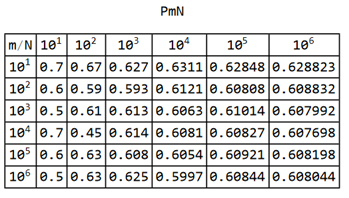
\includegraphics[width=10cm]{2_1.png} \\
        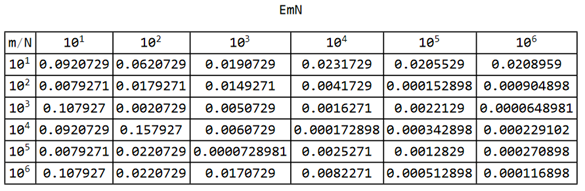
\includegraphics[width=15cm]{2_2.png} \\

        Podemos concluir a partir da tabela EmN que o erro absoluto vai diminuindo de forma consistente à medida que usamos mais números significativos, ou seja, à medida que aumentamos a precisão. Deste modo, é seguro afirmar que as tabelas confirmam a fórmula (1).

        Notas:
        \begin{itemize}
            \item O código demora cerca de 10 segundos a correr.
            \item Sendo os valores dependem de probabilidades, estes variam sempre que corremos o código.
            \item Os valores para o erro não estão 100\% alinhados com o que deveria acontecer (por exemplo, o erro de alguns casos comparado com outros é menor, apesar de os graus de grandeza serem menores), mas considerando que este método é aleatório também é de esperar que haja ligeiras inconsistências. Contudo, analisando de um modo geral, os valores estão perto do esperado (à medida que nos aproximamos do canto inferior direito da tabela, o valor do erro vai diminuindo).
        \end{itemize}

    \subsection{e)}
        Para esta pergunta começámos por criar a função “Pm”, que é simplesmente a fórmula no enunciado, e calculámos para os diferentes valores de m pedidos. De seguida, determinámos os erros para cada m (tal como no exercício anterior) e criámos a lista “Em” com todos estes valores. Criámos ainda uma lista “k”, que vai ser útil para os valores das abcissas do gráfico, sendo que estes valores correspondem aos graus de grandeza. A lista “variables” serve para associar as coordenadas x (“k”) e y (“Log[10, Em]”) de cada ponto usando a função Transpose. Por fim, usámos a função ListPlot para construir o gráfico (com a lista anterior), ligámos os pontos com linhas para facilitar a visualização e indicámos os intervalos mais aconselháveis para a observação do mesmo. \\

        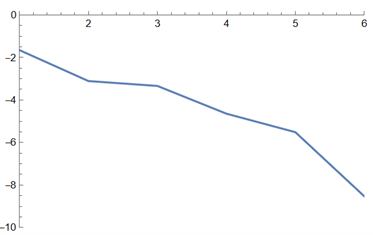
\includegraphics[width=8cm]{2_3.png} \\
        
        Sendo que o erro tende para 0, então o logaritmo do erro também vai tender para \(-\infty\), que é exatamente o que acontece no gráfico. Logo, este gráfico confirma a validade da fórmula (2).
    
    \newpage
    \section{3. Formiga de Langton}
    \subsection{a)}
        A função LangtonsAnt é definida com três argumentos: um inteiro \texttt{n} tal que a matriz que representa a grelha tem dimensão \((2n+1) \times (2n+1)\); uma string \texttt{d}, que pode tomar os valores "Cima", "Baixo", "Esquerda" ou "Direita", definindo a direção inicial da formiga; e um inteiro \texttt{kmax}, correspondente ao número máximo de passos permitido. A função é definida utilizando o comando \texttt{Module}, que permite a declaração de variáveis locais.
        
        Inicialmente, definem-se duas funções internas, \texttt{rotateClockWise} e \texttt{rotateCounterclockWise}, que, dado um vetor, retornam o resultado de lhe aplicar uma rotação de 90º no respetivo sentido.
        
        De seguida, inicializa-se a grelha como um \texttt{ConstantArray}, com o tamanho calculado por \(2n+1\) e com todos os valores a zero. Para além disso, é inicializada a variável que representa a direção como o vetor (lista com 2 elementos) a partir da cadeia de caracteres que a função recebe como argumento.
        
        Finalmente, entra-se no while loop que fará a evolução dos vários estados da grelha. Identifica-se a cor da célula atual, para se alterar a direção de acordo com a regra correspondente, e, de seguida, atualiza-se a cor da célula atual e altera-se a posição para a célula seguinte. Este ciclo corre até que a formiga atinja a a fronteira da grelha ou se chegue ao número máximo de passos, \texttt{kmax}.

    \subsection{b)}
        A aplicação da função definida em a) para \(k_{max}\) = \{250, 500, 750, 1000\}, com valores \(n = 12\) e \(d = "Direita"\) (sendo o valor de \(n\) escolhido de forma a ter uma boa visualização e a não ocorrer o fim do ciclo por atingimento da fronteira), mostra os seguintes resultados: \\
        
        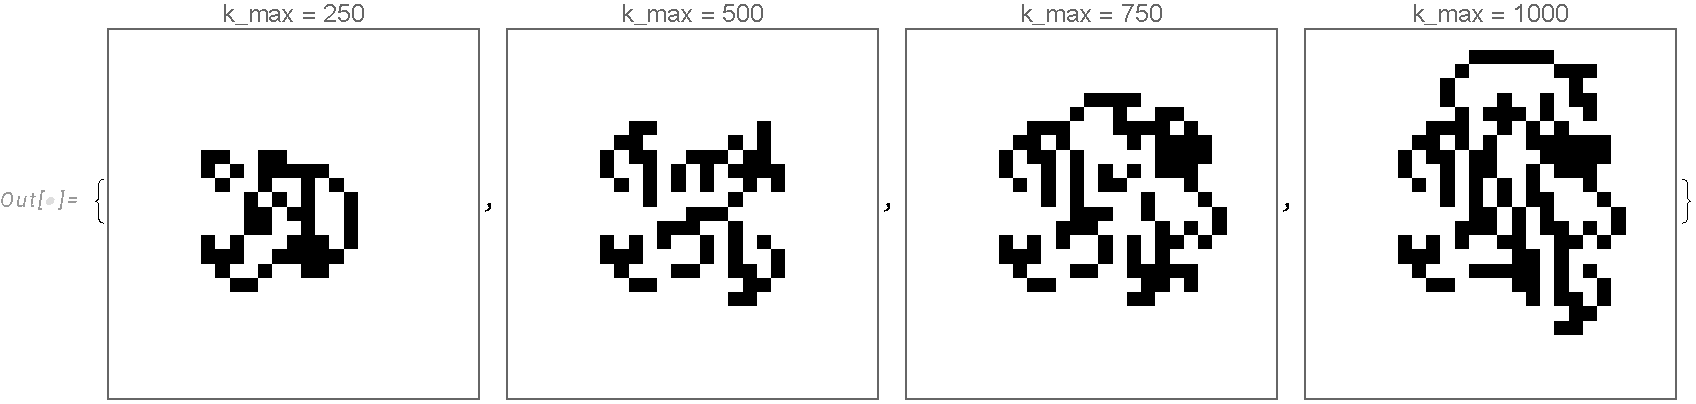
\includegraphics[width=17cm]{3b_1.pdf}

        A aplicação da função para \(k_{max}\) = \{9000, 9500, 10000, 10500, 11000\}, com valores \(n = 38\) e \(d = "Direita"\) (sendo \(n\) escolhido com o critério anterior), mostra os seguintes resultados: \\

        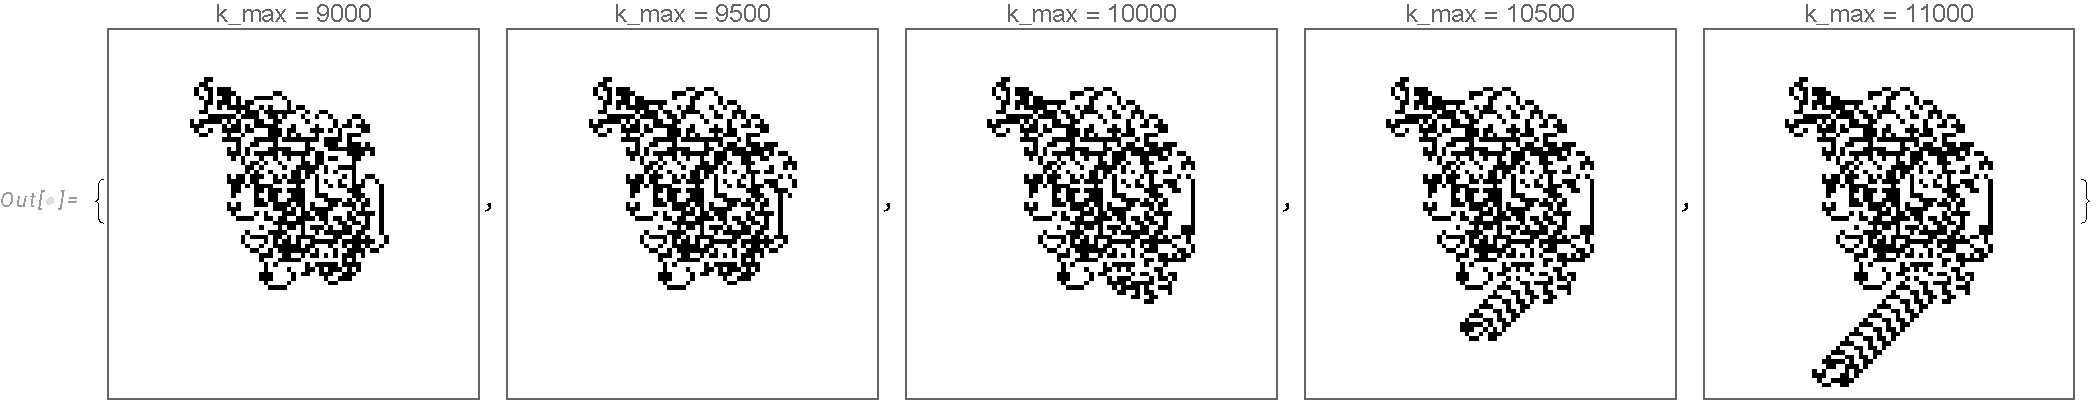
\includegraphics[width=17cm]{3b_2.pdf}

        É possível verificar que, neste intervalo de valores de \(k_{max}\), se chega a um ponto em que a formiga passa a descrever um padrão específico, fenómeno este que se analisará de seguida.

    \subsection{c)}
        Altera-se a função definida em a), de forma a que o seu output não seja apenas a grelha final, mas também a direção final. Isto deve-se ao facto de que o movimento com padrão específico é periódico a menos de translação, ou seja, para identificar e estudar o padrão, a variável de interesse é a direção final da formiga no fim do ciclo para cada valor de \(k_{max}\).

        Encontra-se o padrão utilizando-se os mesmos valores de \(n = 38\) e \(d = "Direita"\), e valores de \(k_{max}\) no intervalo de 10000 a 11000.

        As grelhas resultantes dos valores de \(k_{max}\) de 10000 (inicial) e 11000 (final) são as seguintes: \\

        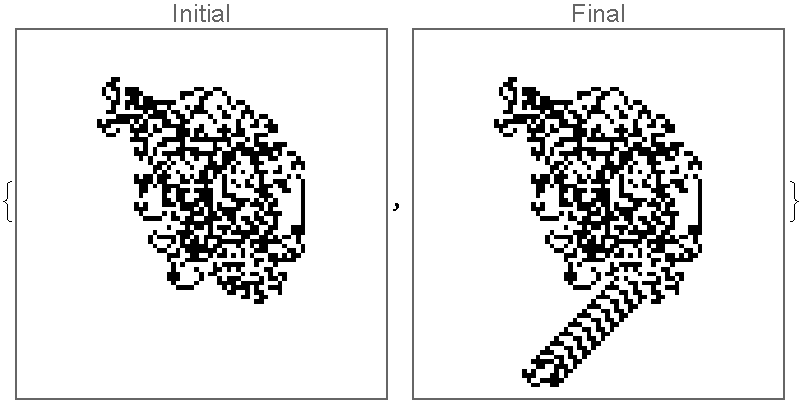
\includegraphics[width=17cm]{3c_1.pdf}

        Utilizando-se o comando \texttt{FindRepeat} para a lista das direções finais das chamadas à função para todos os valores de \(k_{max}\) entre o valor inicial e o final, obtém-se o seguinte padrão:

        \begin{verbatim}
{{0,1},{1,0},{0,-1},{1,0},{0,-1},{1,0},{0,1},{-1,0},{0,-1},{-1,0},{0,-1},{-1,0},
{0,1},{1,0},{0,-1},{1,0},{0,1},{-1,0},{0,-1},{-1,0},{0,-1},{1,0},{0,-1},{1,0},
{0,1},{-1,0},{0,-1},{-1,0},{0,1},{1,0},{0,-1},{1,0},{0,-1},{1,0},{0,1},{-1,0},
{0,-1},{-1,0},{0,-1},{1,0},{0,1},{-1,0},{0,1},{1,0},{0,-1},{-1,0},{0,-1},{-1,0},
{0,-1},{1,0},{0,1},{-1,0},{0,1},{-1,0},{0,1},{1,0},{0,1},{-1,0},{0,1},{1,0},
{0,-1},{-1,0},{0,-1},{1,0},{0,-1},{-1,0},{0,-1},{1,0},{0,1},{-1,0},{0,1},{1,0},
{0,1},{-1,0},{0,1},{-1,0},{0,1},{1,0},{0,1},{1,0},{0,-1},{1,0},{0,-1},{1,0},
{0,-1},{-1,0},{0,-1},{1,0},{0,1},{-1,0},{0,1},{1,0},{0,1},{1,0},{0,-1},{1,0},
{0,1},{-1,0},{0,-1},{-1,0},{0,1},{-1,0},{0,-1},{1,0}}
        \end{verbatim}

        Através do comando \texttt{Length}, obtém-se o comprimento desta lista, concluindo-se que o período mínimo deste movimento periódico é de 104.

    \newpage
    \subsection{d)}
        A função definida em a) é alterada, passando agora a ter mais um argumento, a cadeia de caracteres com as regras do sistema, que definem, para cada possível cor de uma célula, qual o sentido da rotação a aplicar na direção da formiga. É também a partir do comprimento desta string que se encontra o número de cores.

        O ciclo da função é alterado. Este continua a alterar a direção de acordo com a regra correspondente à cor da célula atual e a atualizar a cor da célula atual, tal como anteriormente, mas o procedimento para o fazer é mais complexo, dado o maior número de cores. As cores são identificadas por inteiros a começar em 0, pelo que, para se obter a cor seguinte, se utiliza o comando \texttt{Mod}.

        A aplicação da função alterada para \(k_{max}\) = 500000, com valores \(n = \{50, 80, 700\}\) e \(d = "Direita"\) (sendo, uma vez mais, os valores de \(n\) escolhidos de forma a não ocorrer o fim do ciclo por atingimento da fronteira), mostra os seguintes resultados: \\
        
        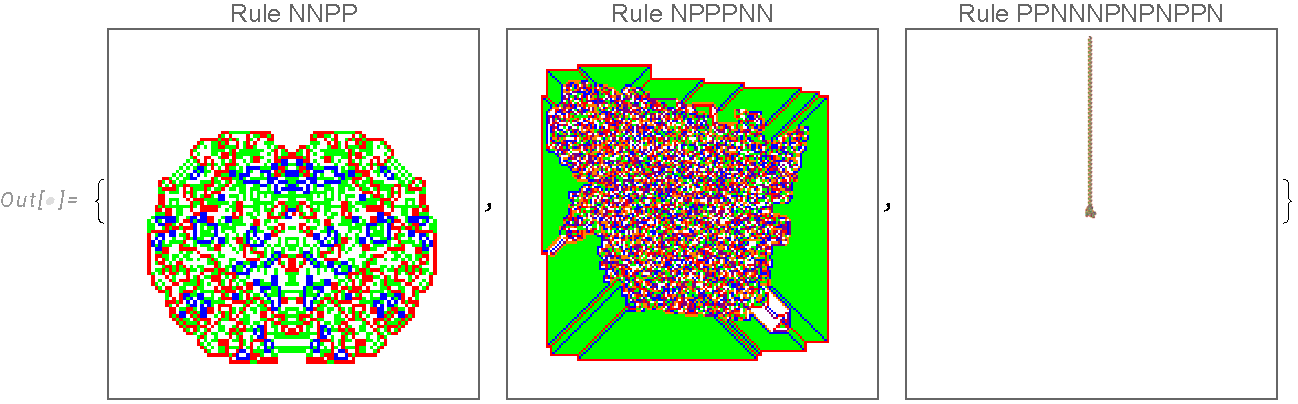
\includegraphics[width=17cm]{3d_1.pdf} \\

        Para a regra "PPNNNPNPNPPN", a visualização fica comprometida pelo formato vertical da trajetória da formiga, pelo que se apresenta de seguida uma ampliação no centro com rotação de 90º no sentido horário dessa imagem: \\

        
\includegraphics[width=17cm]{3d_2.png} \\

        Verifica-se que, a partir de um certo ponto, a trajetória da formiga passa a descrever um movimento com padrão específico.

\end{document}